\documentclass[11pt]{article}
\usepackage[utf8]{inputenc}
\usepackage[brazilian]{babel}
\usepackage{graphicx}
\usepackage[a4paper, top={.4in}, bottom={.65in}]{geometry}
\usepackage{subfig}
\usepackage{makecell}
\usepackage{textcomp}
\usepackage{gensymb}
\usepackage{tikz}
\usepackage{amsmath}
\usepackage{amssymb}
\usepackage{upgreek}
\usepackage{booktabs}
\usepackage{indentfirst}

\begin{document}

\begin{center}
  \textbf{Experimento 09 -- PSI-3212} \\
  Natanael Magalhães Cardoso, nUSP: 8914122
\end{center}

\subsection*{Item 1.a}

\begin{figure}[h!]
  \centering
  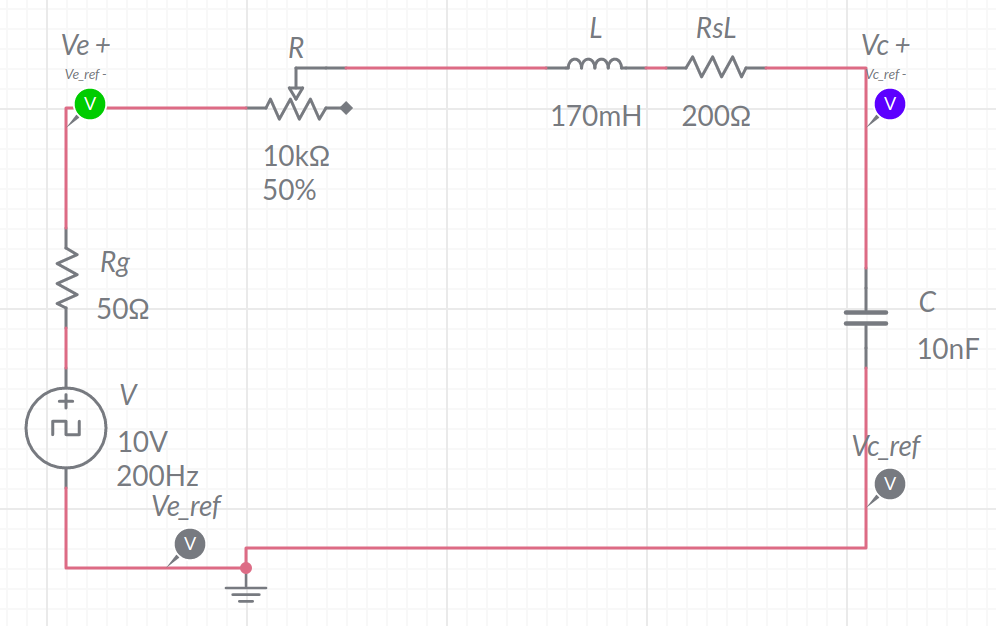
\includegraphics[width=.6\textwidth]{fig/1-circ}
  \caption{Esquema do circuito.}
  \label{fig:1-circ}
\end{figure}

\begin{figure}[h!]
  \centering
  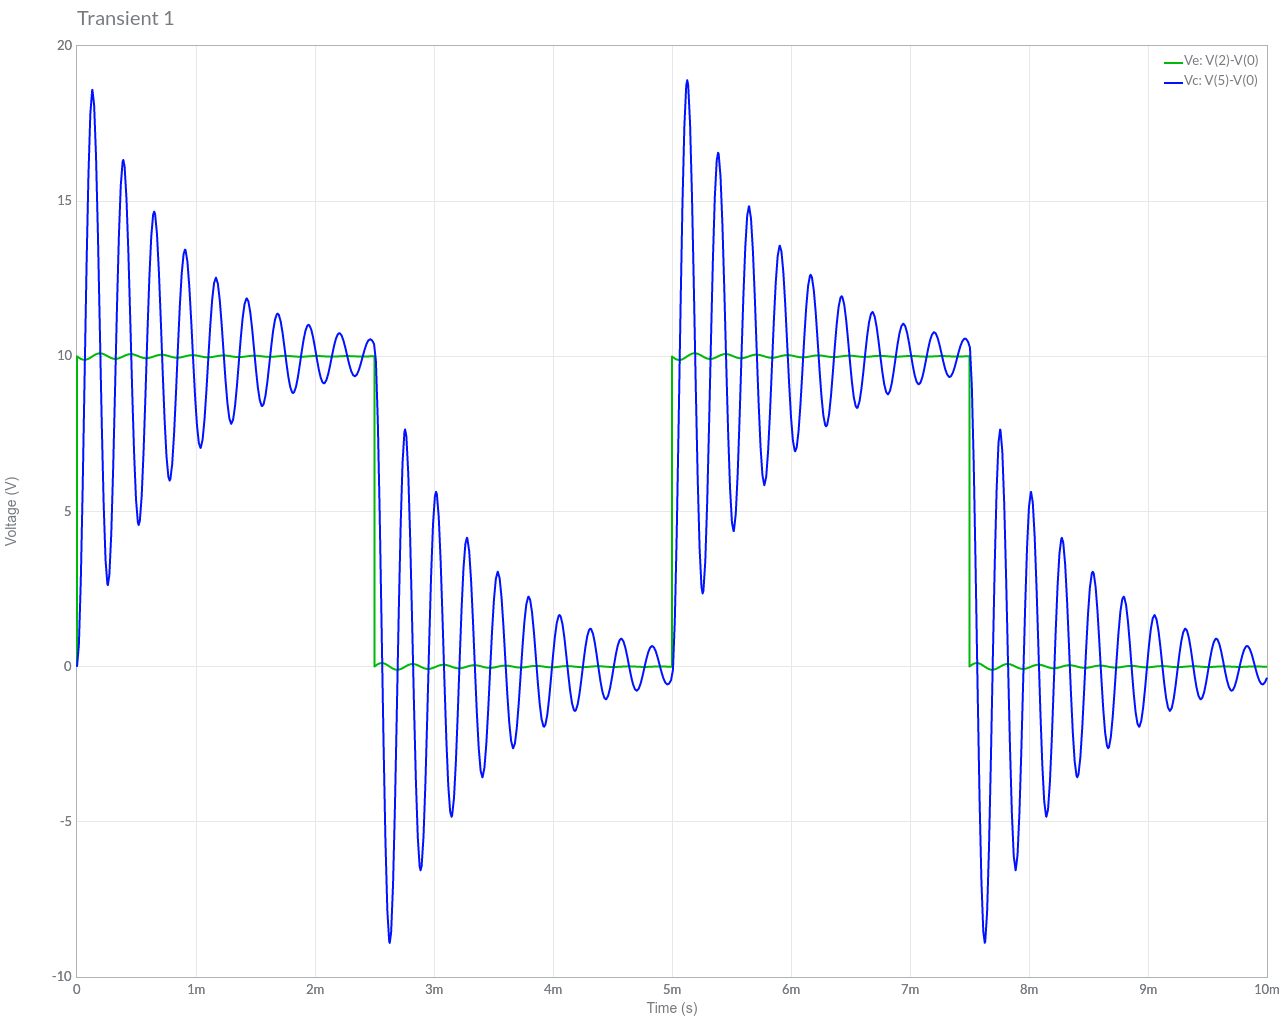
\includegraphics[width=.6\textwidth]{fig/1a-1}
  \caption{Simulação para $V_{e}$ e $V_{c}$ com o potenciômetro ajustado em 150 $\Omega$.}
  \label{fig:1a-1}
\end{figure}

\begin{figure}[h!]
  \centering
  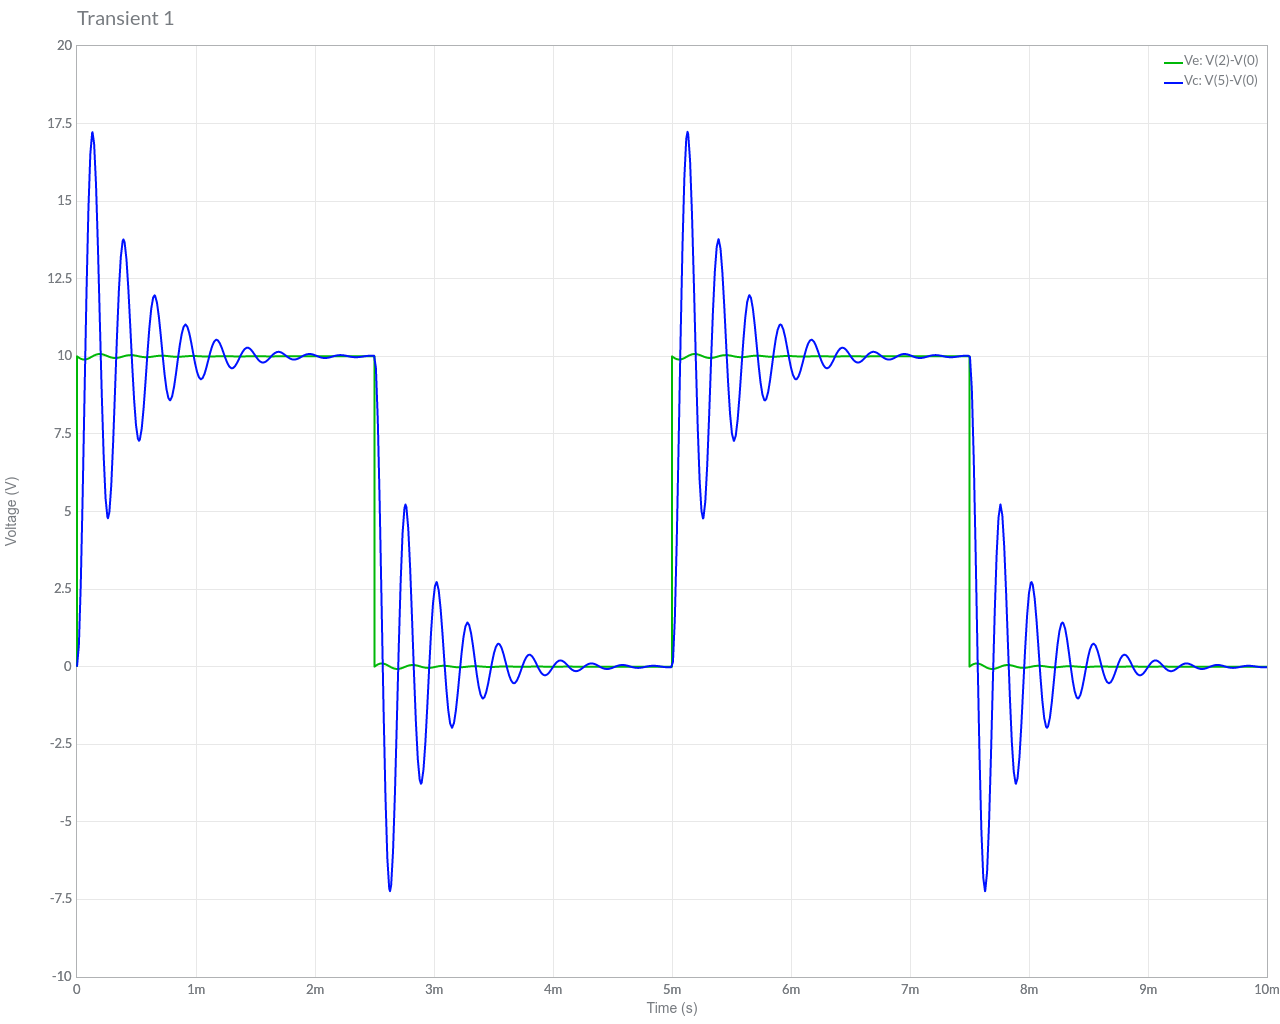
\includegraphics[width=.6\textwidth]{fig/1a-2}
  \caption{Simulação para $V_{e}$ e $V_{c}$ com o potenciômetro ajustado em 600 $\Omega$.}
  \label{fig:1a-2}
\end{figure}

\begin{figure}[h!]
  \centering
  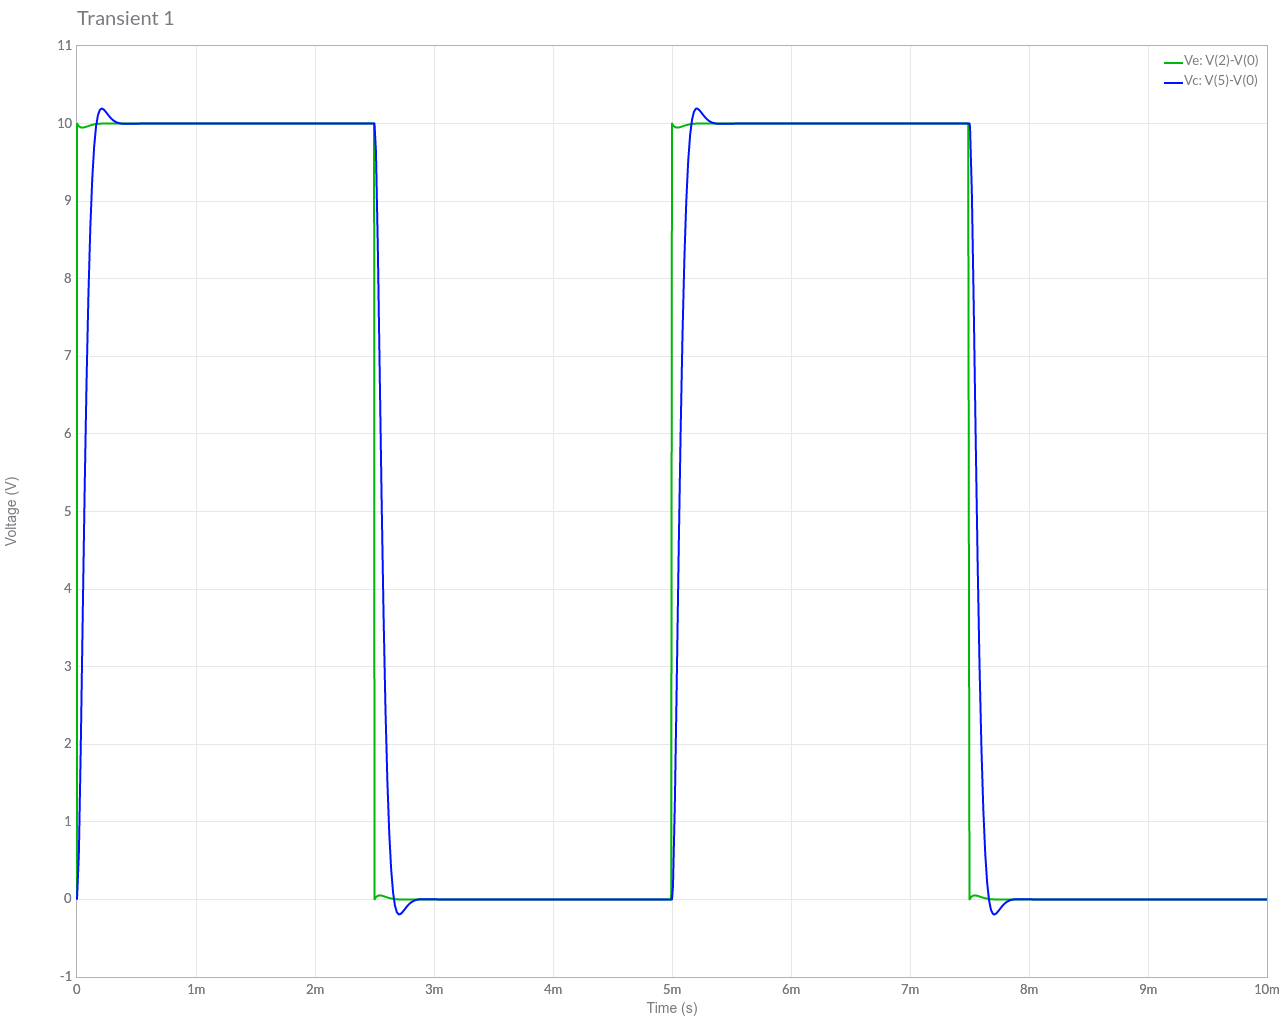
\includegraphics[width=.6\textwidth]{fig/1a-3}
  \caption{Simulação para $V_{e}$ e $V_{c}$ com o potenciômetro ajustado em 6.2 k$\Omega$.}
  \label{fig:1a-3}
\end{figure}

\begin{figure}[h!]
  \centering
  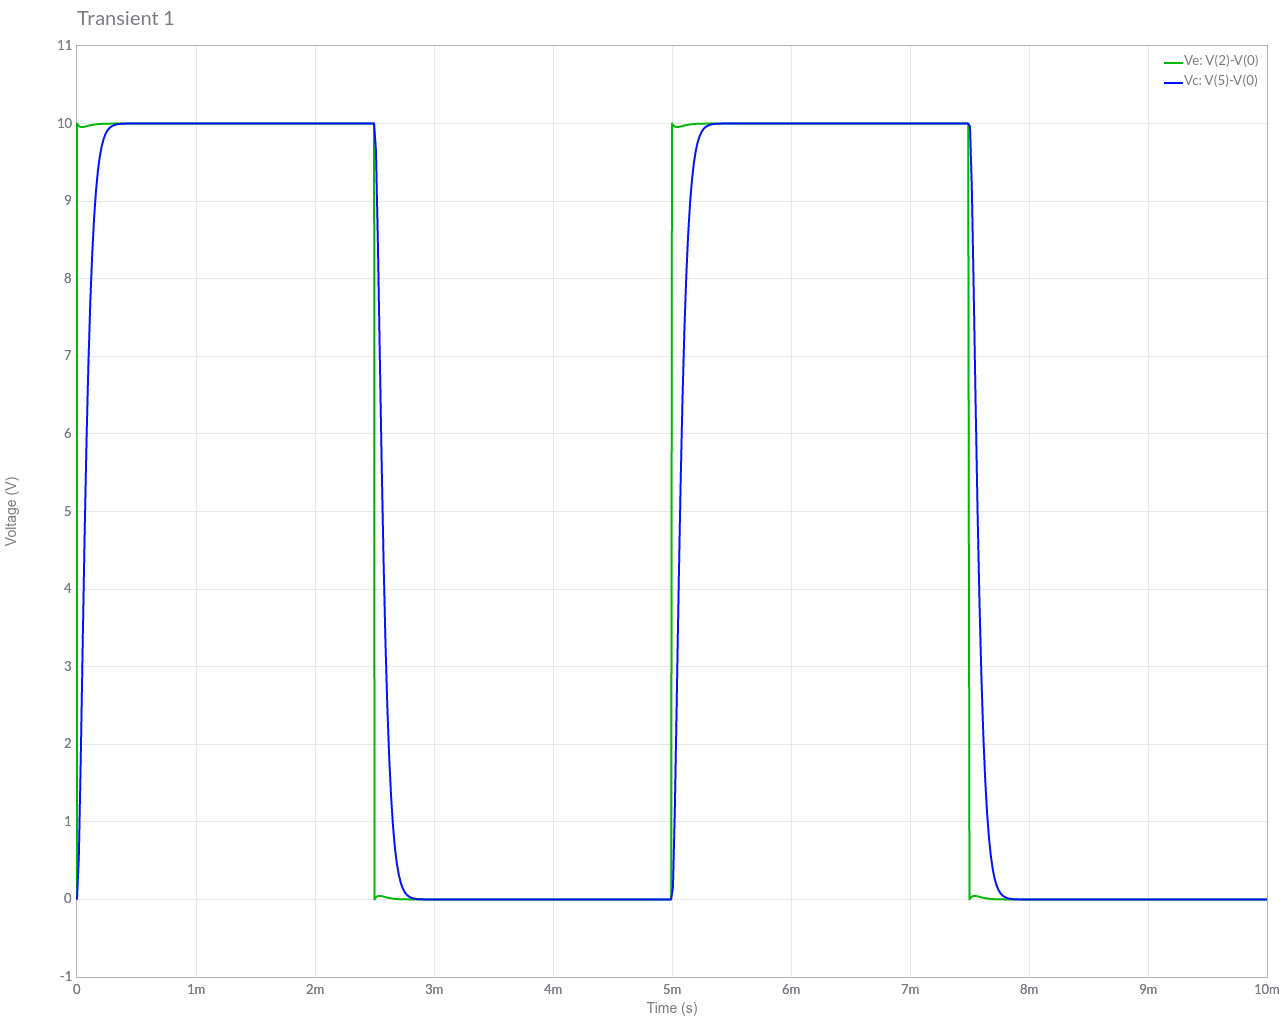
\includegraphics[width=.6\textwidth]{fig/1a-4}
  \caption{Simulação para $V_{e}$ e $V_{c}$ com o potenciômetro ajustado em 7.7 k$\Omega$.}
  \label{fig:1a-4}
\end{figure}

\begin{figure}[h!]
  \centering
  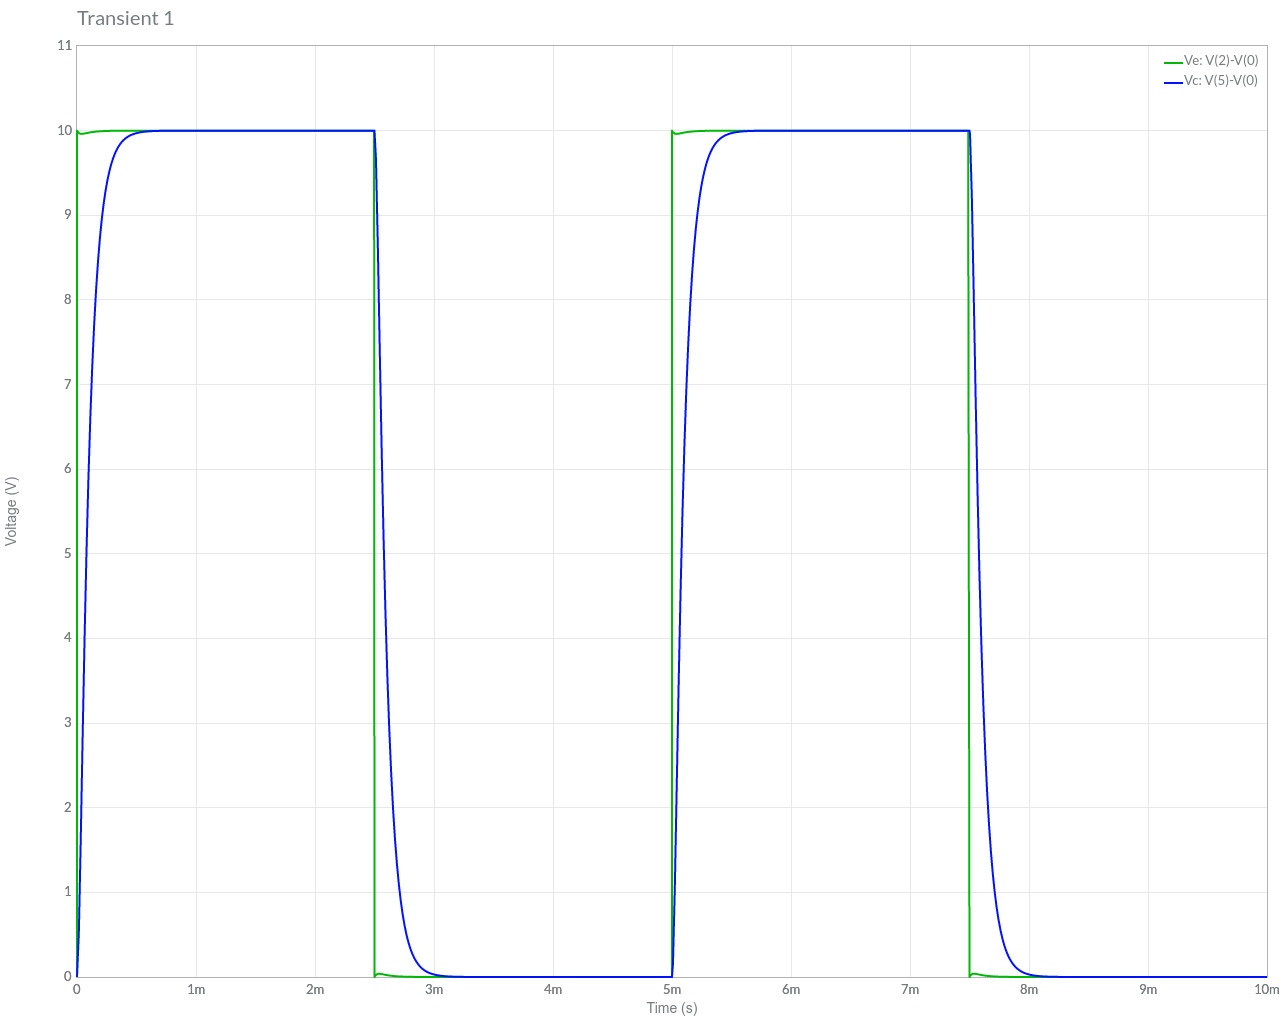
\includegraphics[width=.6\textwidth]{fig/1a-5}
  \caption{Simulação para $V_{e}$ e $V_{c}$ com o potenciômetro ajustado em 10 k$\Omega$.}
  \label{fig:1a-5}
\end{figure}

\subsection*{Item 1.b}

Nas figuras \ref{fig:1a-1}, \ref{fig:1a-2} e \ref{fig:1a-3}, as curvas de $V_{c}$ apresentam um regime amortecido ou subamortecido, sendo que, no primeiro caso, a tensão demora mais tempo para estabilizar-se que o tempo de inversão do sinal da fonte. A tensão $V_{c}$ na figura \ref{fig:1a-4} está mais próxima de uma resposta criticamente amortecida enquanto a curva da figura \ref{fig:1a-5} aproxima-se mais de um regime superamortecido, por demorar mais para estabilizar-se com a tensão da fonte. Em ambos os casos, a tensão do capacitor sempre tende a estabilizar-se com tensão de entrada (fonte).

\subsection*{Item 2.a}

\begin{figure}[h!]
  \centering
  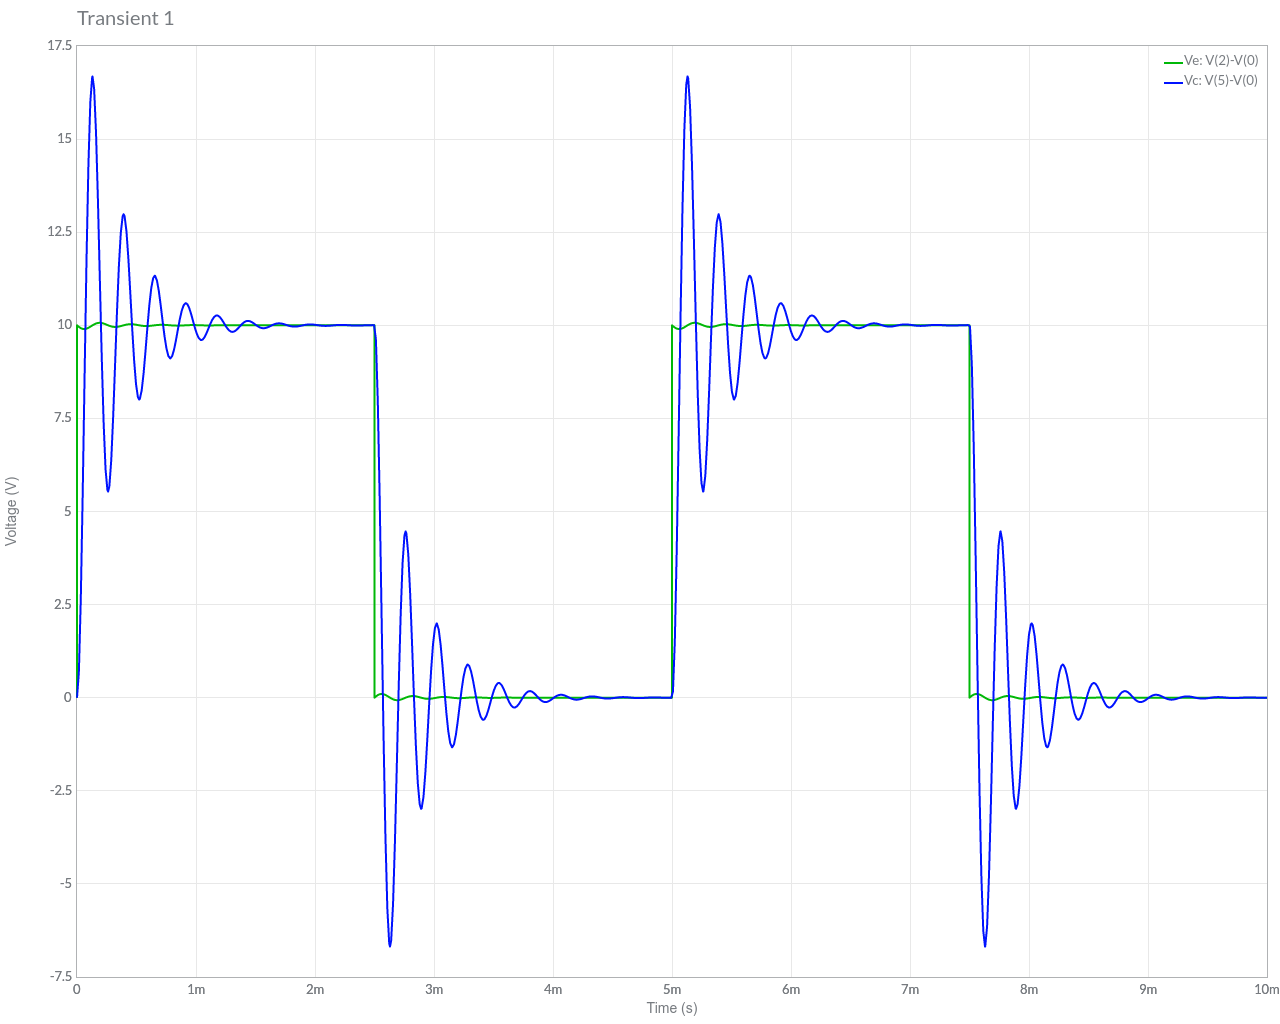
\includegraphics[width=.75\textwidth]{fig/2a}
  \caption{Simulação para regime subamortecido.}
  \label{fig:2a}
\end{figure}

$$
  R_{p} = 800\ \Omega
$$

$$
  R_{eq} = R_{p} + R_{g} + R_{sL} = (800 + 50 + 200)\ \Omega = 1.05\ k\Omega
$$

\subsection*{Item 2.b}

\begin{figure}[h!]
  \centering
  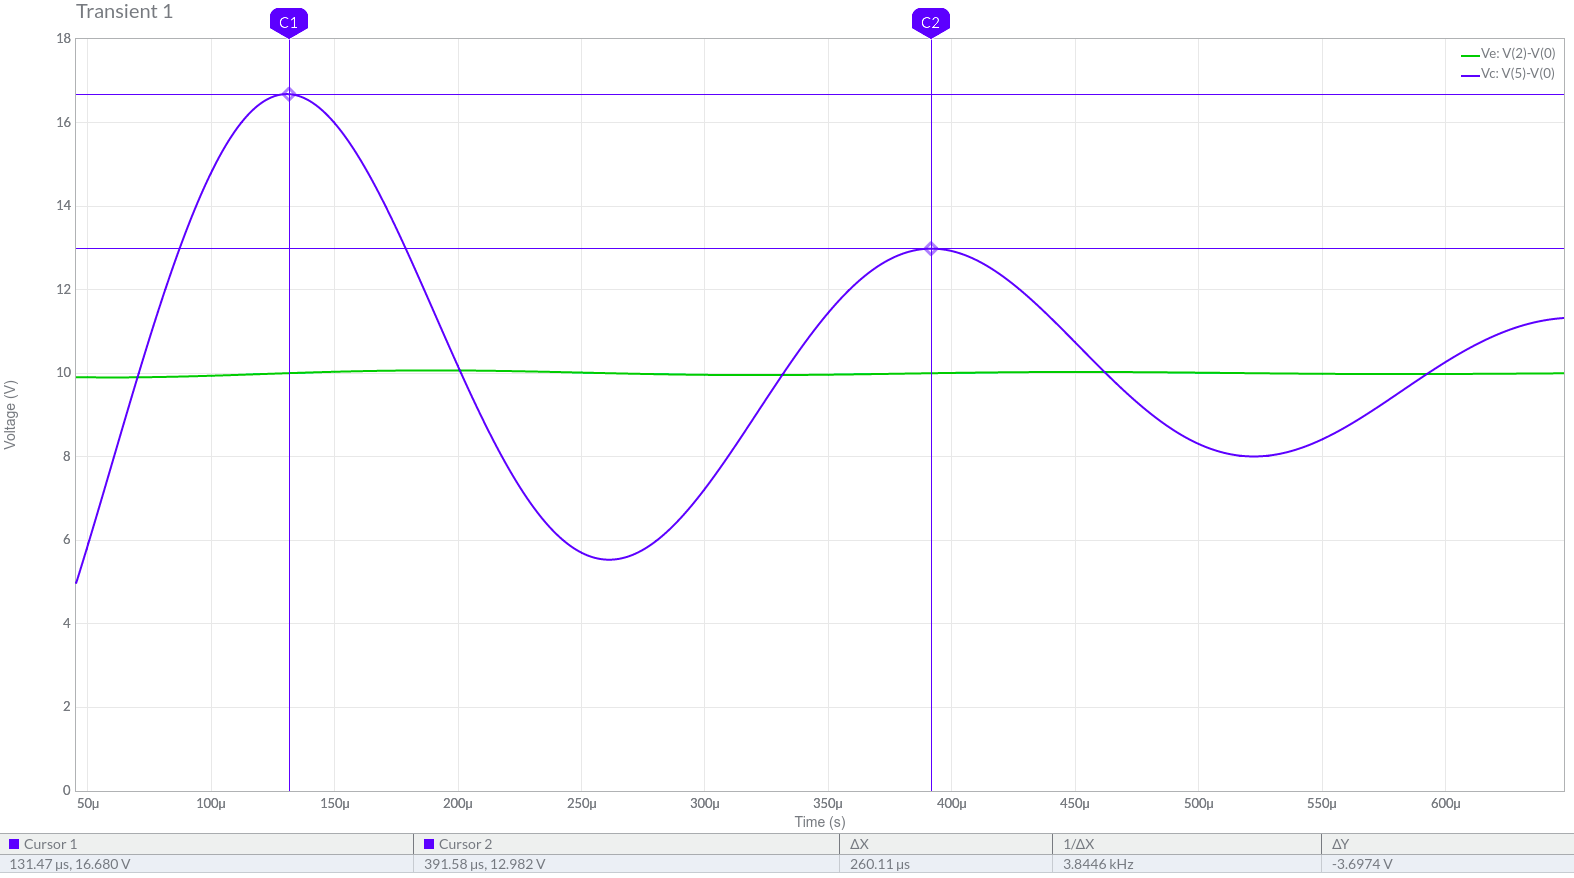
\includegraphics[width=\textwidth]{fig/2b}
  \caption{Período de oscilação.}
  \label{fig:2b}
\end{figure}

Do simulador: $\Delta x = T = 260.11\ \mu\text{s}$, então:

$$
  \omega_{d} = \frac{2\pi}{T} = \frac{2\pi}{\Delta x} = \frac{2\pi}{260.11\ \mu\text{s}} = 24155.88\ \text{rad/s}
$$

\subsection*{Item 2.c.1}

\begin{figure}[h!]
  \centering
  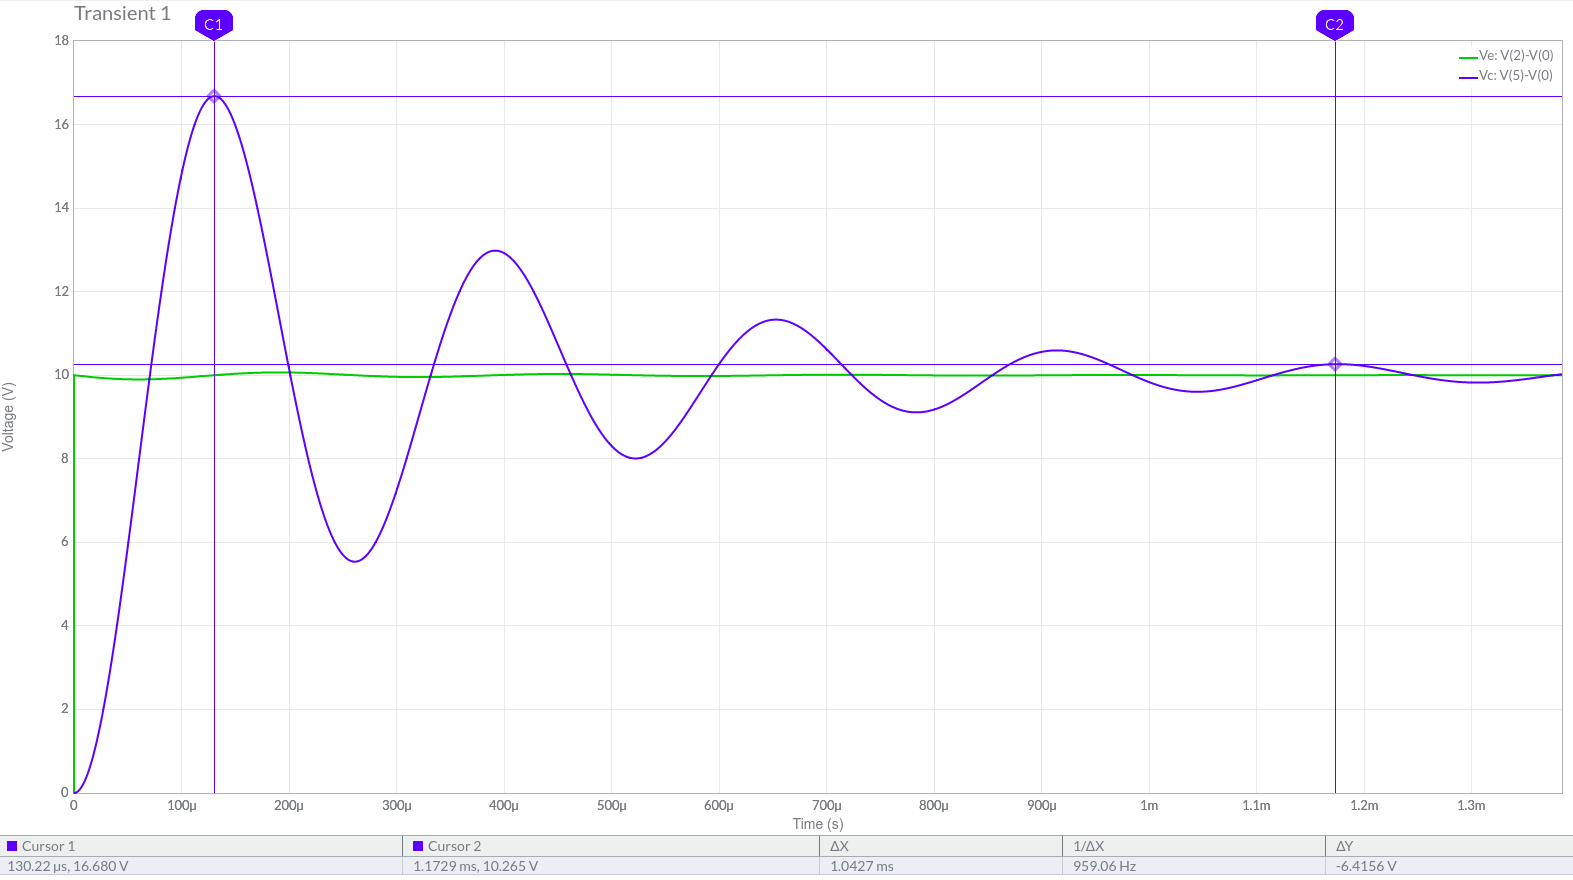
\includegraphics[width=\textwidth]{fig/2c1}
  \caption{Valores para primeiro e quinto pico da oscilação.}
  \label{fig:2c1}
\end{figure}

\subsection*{Item 2.c.2}

\begin{table}[h!]
  \centering
  \begin{tabular}{|c|c|c|}
    \hline
    n & $A_{n}$ (V) & $t_{n}$        \\
    \hline
    1 & 6.680       & 130.22  $\mu$s \\
    5 & 0.265       & 1.17  ms       \\
    \hline
  \end{tabular}
  \caption{Valores medidos na simulação da figura \ref{fig:2c1}. $A_{n}$ calculado usando $A_{n} = V_{c} - V_{e}$.}
  \label{tab:2c2}
\end{table}

\subsection*{Item 2.c.3}

Da definição de logarítmo:

\begin{equation}
  \log_\beta x = \alpha \; \Leftrightarrow \; \beta^x = \alpha
  \label{eq:def-log}
\end{equation}

Da expressão da amplitude:

\begin{equation}
  A(t) {}={} A_0 e^{-\alpha t} \; \Rightarrow \; e^{-\alpha t} {}={} \frac{A(t)}{A_0}
  \label{eq:ampl}
\end{equation}

\eqref{eq:def-log} $\rightarrow$ \eqref{eq:ampl}:

$$
  -\alpha t = \ln \left(\frac{A(t)}{A_0}\right) \; \Rightarrow \; \alpha = - \frac{1}{t} \ln \left(\frac{A(t)}{A_0}\right)
$$

A curva de A(t) da figura \ref{fig:2c3} mostra o gráfico da amplitude em função do tempo $A(t) = A_0 e^{-\alpha t}$ para $A_0$ = $V_g$ = 10 V e $\alpha = \alpha_{exp}$. Ou seja, $A(t) = 10 e^{-3103.68 t}$ [V].

\pagebreak

\begin{figure}[h!]
  \centering
  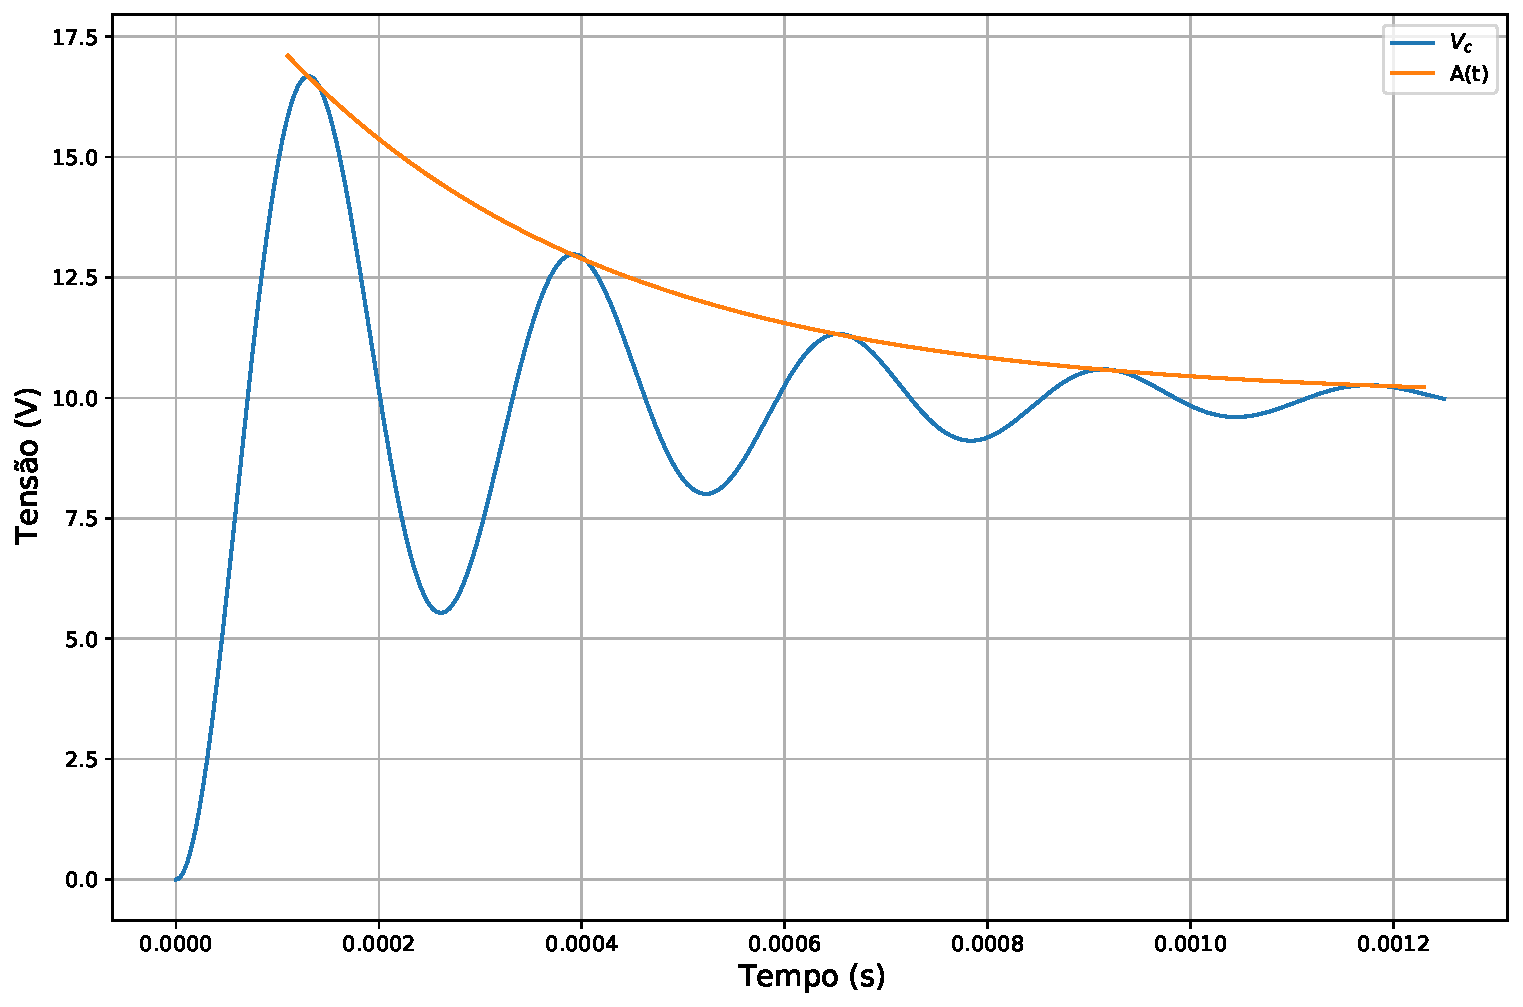
\includegraphics[width=\textwidth]{fig/2c3}
  \caption{Curva A(t) e tensão $V_c$.}
  \label{fig:2c3}
\end{figure}

\subsection*{Item 2.c.4}

Para $A_n = 0.265$ V, $A_0 = 6.68$ V, $\Delta t = t_5 - t_1 = 1.04$ ms

$$
  \alpha_{exp} = - \frac{1}{1.04} \ln \left(\frac{0.265}{6.68}\right) = 3103.68\ \text{rad/s}
$$

Para $R_{eq}$ = 1.05 k$\Omega$ e L = 170 mH

$$
  \alpha_{teo} = \frac{R_{eq}}{2L} = \frac{1.05 \cdot 10^3\ \Omega}{2 \cdot 170 \cdot 10^{-3}\ \text{H}} = 3088.24\ \text{rad/s}
$$

\subsection*{Item 3}

$$
  R_p = 7.2\ \text{k}\Omega \qquad \qquad R_{eq} = 7.45\ \text{k}\Omega
$$

\begin{figure}[h!]
  \centering
  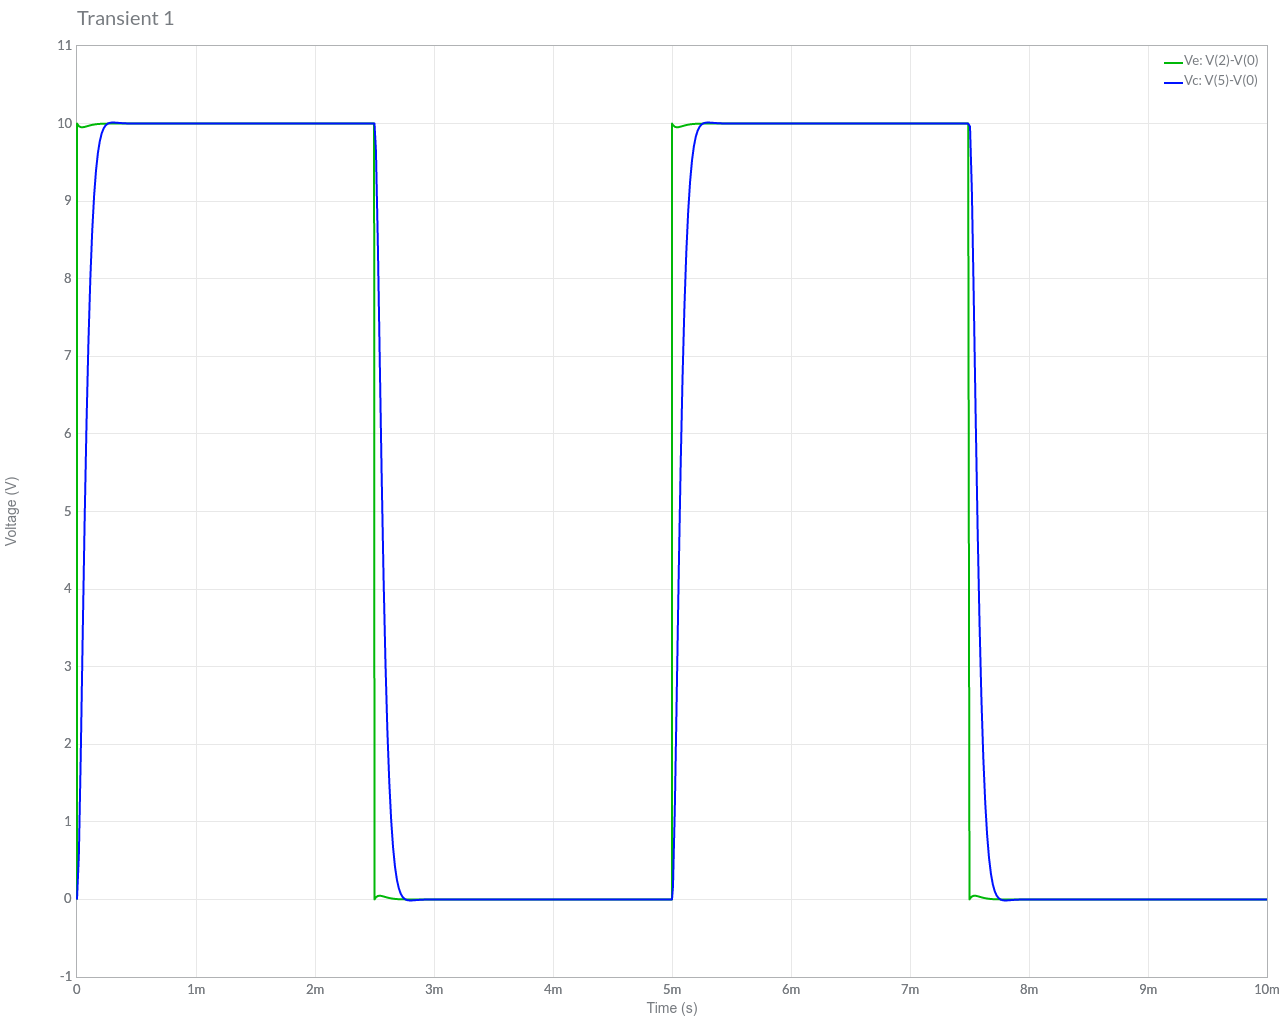
\includegraphics[width=.6\textwidth]{fig/3}
  \caption{Simulação para 7.2 k$\Omega$ de resistência no potenciômetro.}
  \label{fig:3}
\end{figure}

\subsection*{Item 4.a}

$$
  R_p = 9.2\ \text{k}\Omega \qquad \qquad R_{eq} = 9.45\ \text{k}\Omega
$$

\begin{figure}[h!]
  \centering
  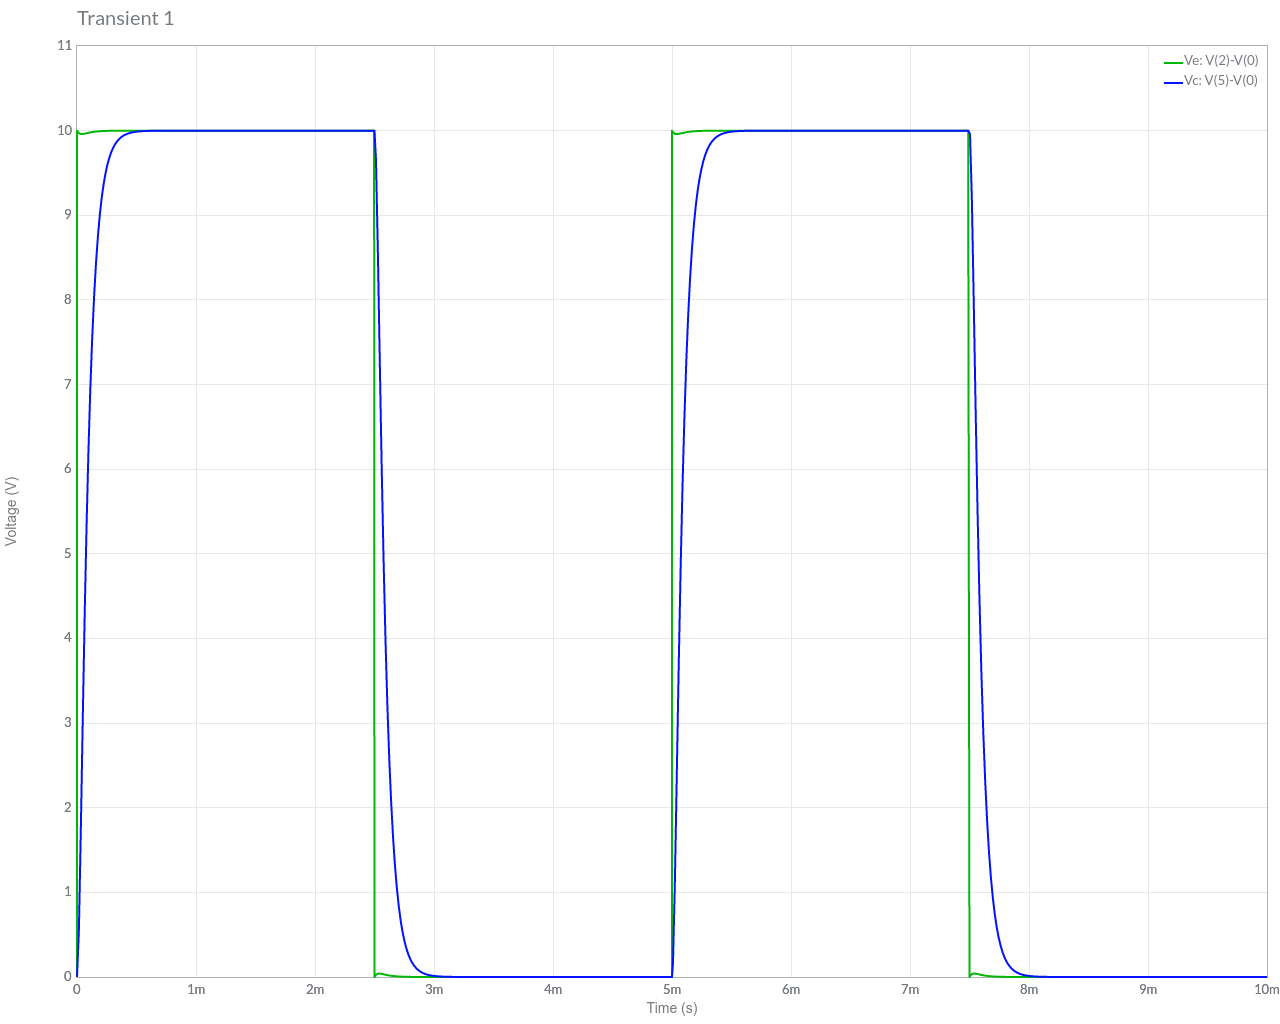
\includegraphics[width=.6\textwidth]{fig/4a}
  \caption{Simulação para 9.2 k$\Omega$ de resistência no potenciômetro.}
  \label{fig:3}
\end{figure}

\subsection*{Item 4.b}

Pelas equações teóricas de $\alpha$ e $\omega$:

$$
  \alpha^2 = \frac{R^2}{4L^2} \qquad \qquad \omega^2 = \frac{1}{LC}
$$

Temos, portanto, os valores:

$$
  \alpha^2 = \frac{(9.45 \cdot 10^3\ \Omega)^2}{4 \cdot (170 \cdot 10^{-3}\ \text{H})^2} = 772.51 \cdot 10^6\ \text{rad/s}
$$

$$
  \omega^2 = \frac{1}{(170 \cdot 10^{-3}\ \text{H})(10 \cdot 10^{-9}\ \text{F})} = 588.24 \cdot 10^6\ \text{rad/s}
$$

Como $\omega^2 < \alpha^2$, o regime é superamortecido. No amortecimento crítico, onde $\omega^2 = \alpha^2$, por outro lado, a tensão $V_c$ estabiliza-se mais rápido.

\end{document}
